% =========================================================================== %
% The Scout Client
% =========================================================================== %

\ifx\wholebook\relax\else
  \documentclass[a4paper,10pt,twoside]{book}
  %=============================================================================%
% Common things, settings, packages to include
%=============================================================================%

\usepackage{graphicx}
\usepackage{color}
\usepackage{makeidx}
\usepackage{ifpdf}
\usepackage{verbatim}

% --------------------------------------------------------------------------- %
% Setting up stuff depeding on output format
% --------------------------------------------------------------------------- %

\ifpdf
  % special settings for pdf mode
  \usepackage[colorlinks]{hyperref}
  \usepackage{courier}
  
  \hypersetup{
    colorlinks,
    linkcolor=darkblue,
    citecolor=darkblue,
    pdftitle={The Eclipse Scout Book},
    pdfauthor={The Scout Community},
    pdfkeywords={Enterprise Framework, Eclipse, Java, Client-Side, Rich Client, Web Client, Mobile},
    pdfsubject={Computer Science}
  }
  
  \usepackage{caption}
  \captionsetup{margin=10pt,font=small,labelfont=bf}
\else
  % special stuff for html mode
  \usepackage[tex4ht]{hyperref}
\fi

% --------------------------------------------------------------------------- %
% Setting up printing range
% --------------------------------------------------------------------------- %

\parindent 1cm
\parskip 0.2cm
\topmargin 0.2cm
\oddsidemargin 1cm
\evensidemargin 0.5cm
\textwidth 15cm
\textheight 21cm

% --------------------------------------------------------------------------- %
% Setting up listings
% --------------------------------------------------------------------------- %

\usepackage{listings}
 
\definecolor{darkviolet}{rgb}{0.5,0,0.4}
\definecolor{darkgreen}{rgb}{0,0.4,0.2} 
\definecolor{darkblue}{rgb}{0.1,0.1,0.9}
\definecolor{darkgrey}{rgb}{0.5,0.5,0.5}
\definecolor{lightblue}{rgb}{0.4,0.4,1}
\definecolor{lightgray}{rgb}{0.97,0.97,0.97}

\renewcommand{\lstlistlistingname}{List of Listings}

% general settings
\lstset{
  basicstyle=\small\ttfamily,
  columns=fullflexible,
  breaklines=true,
  breakindent=10pt,
  prebreak=\mbox{{\color{blue}\tiny$\searrow$}},
  postbreak=\mbox{{\color{blue}\tiny$\rightarrow$}},
  showstringspaces=false,
  backgroundcolor=\color{lightgray}
}

% settings for xml files
\lstdefinelanguage{xml}
{
  commentstyle=\color{darkgrey}\upshape,
  morestring=[b]",
  morestring=[s]{>}{<},
  morecomment=[s]{<?}{?>},
  stringstyle=\color{black},
  identifierstyle=\color{darkblue},
  keywordstyle=\color{cyan},
  morekeywords={xmlns,name,point,factory,class}% list your attributes here
}

% settings for ini files
\lstdefinelanguage{ini}
{
  morecomment=[f][\color{darkgrey}\upshape][0]\#, % # is comment iff it's the first char on the line
  stringstyle=\color{black}
}

% default settings (for java files)
\lstset{
  language=Java,
  emphstyle=\color{red}\bfseries,
  keywordstyle=\color{darkviolet}\bfseries,
  commentstyle=\color{darkgreen},
  morecomment=[s][\color{lightblue}]{/**}{*/},
  stringstyle=\color{darkblue},
}

% --------------------------------------------------------------------------- %
% cross reference macros
% --------------------------------------------------------------------------- %
\newcommand{\applabel}[1]{\label{apx:#1}}
\newcommand{\chalabel}[1]{\label{cha:#1}}
\newcommand{\seclabel}[1]{\label{sec:#1}}
\newcommand{\lstlabel}[1]{\label{lst:#1}}
\newcommand{\figlabel}[1]{\label{fig:#1}}
\newcommand{\tablabel}[1]{\label{tab:#1}}

\newcommand{\appref}[1]{Appendix~\ref{apx:#1}}
\newcommand{\charef}[1]{Chapter~\ref{cha:#1}\xspace}
\newcommand{\secref}[1]{Section~\ref{sec:#1}}
\newcommand{\lstref}[1]{Listing~\ref{lst:#1}\xspace}
\newcommand{\figref}[1]{Figure~\ref{fig:#1}\xspace}
\newcommand{\tabref}[1]{Table~\ref{tab:#1}\xspace}

% --------------------------------------------------------------------------- %
% graphics paths
% --------------------------------------------------------------------------- %
\graphicspath{
  {figures/}
  {Introduction/figures/}
}

%=============================================================================%

  \pagestyle{headings}
  \graphicspath{{figures/} {../figures/}}
  \begin{document}
  \sloppy
\fi


% =========================================================================== %
\chapter{Overview}
\chalabel{client_overview}

needs text
  
\noindent Existing Documentation
\begin{itemize}
  \item concept wiki \url{http://wiki.eclipse.org/Scout/Concepts/Client_Plug-In}
\end{itemize}

% --------------------------------------------------------------------------- %
\section{Component Model}
needs text

\noindent Existing Documentation
\begin{itemize}
  \item wiki concept \url{http://wiki.eclipse.org/Scout/Concepts/Client_Plug-In#Component_Model}
  \item concept wiki \url{http://wiki.eclipse.org/Scout/Concepts/ClientSession}
\end{itemize}

  * client session
  * ui
  * other
  
% --------------------------------------------------------------------------- %
\section{Separation of UI Technologies}
needs text

\noindent Existing Documentation
\begin{itemize}
  \item wiki concept \url{http://wiki.eclipse.org/Scout/Concepts/Client_Plug-In#Separation_of_UI_and_GUI}
\end{itemize}
  
  * swing
  * swt
  * rap

\section{Test for Listing}

introductionary listing

\lstinputlisting[
  caption=The DesktopForm.java in the UI,
]
{../code/helloworld/org.eclipse.scout.helloworld.client/src/org/eclipse/scout/helloworld/client/ui/forms/DesktopForm.java}


some text before listing\index{listing} \ref{samplecode}.

\lstinputlisting[
  label=samplecode,
  caption=The HelloWorld.java sample with emphasys on \it{println},
  index={println,main,String},
  float,
  emph={println}
]
{../code/helloworldJava/HelloWorld.java}


\lstinputlisting[
  label=samplecode-main,
  caption=Snippet containing the main method,
  linerange={14-18},
  float
]
{../code/helloworldJava/HelloWorld.java}


some text after listing \ref{samplecode} and \ref{samplecode-main}.

% =========================================================================== %
\chapter{Client Modeling}
\chalabel{client_modeling}

needs text. this should be a complete chapter as the client modeling is one
of scouts key features.

internal structure to be decided. consequences for other chapters/sections in
this part to be verified

% =========================================================================== %
\chapter{Shared Components}
needs text
  
% --------------------------------------------------------------------------- %
\section{Texts / i18n / NLS Support}
needs text

\noindent Existing Documentation
\begin{itemize}
  \item concept wiki: \url{http://wiki.eclipse.org/Scout/Concepts/Texts}
  \item forum: \url{http://www.eclipse.org/forums/index.php/t/319136/}
  \item forum: \url{http://www.eclipse.org/forums/index.php/t/326343/}
  \item forum: overwriting texts provided by scout \url{http://www.eclipse.org/forums/index.php/t/308273/}
  \item forum: additional text provider service \url{http://www.eclipse.org/forums/index.php/t/317565/}
  \item forum: changing default language for scout apps \url{http://www.eclipse.org/forums/index.php/t/367177/}
  \item forum: export/import not possible: \url{http://www.eclipse.org/forums/index.php/t/326320/}
  \item forum: usage counts for text entries: \url{http://www.eclipse.org/forums/index.php/t/261235/}
\end{itemize}

\begin{lstlisting}[
  float,
  caption=A floating HelloWorld example,
  index={main},
  gobble=2
]
    /*************************************************
     * main method
     *************************************************/
    public static void main(String[] args) {
        // some normal line comment
        System.out.println("Hello, World");
        Some.big().andEspeciallyLong().getThisOrThat().orSomething("string", null).doThis().doThat;
    }
\end{lstlisting}

% --------------------------------------------------------------------------- %
\section{Icons}
needs text

\noindent Existing Documentation
\begin{itemize}
  \item how-to wiki \url{http://wiki.eclipse.org/Scout/HowTo/3.8/Add_an_icon}
  \item how-to wiki \url{http://wiki.eclipse.org/Scout/HowTo/3.8/Exchange_Default_Images}
\end{itemize}

% --------------------------------------------------------------------------- %
\section{Codes and Code Types}
needs text

\noindent Existing Documentation
\begin{itemize}
  \item how-to wiki: \url{http://wiki.eclipse.org/Scout/Tutorial/3.8/Minicrm/Code_Types}
  \item concept wiki \url{http://wiki.eclipse.org/Scout/Concepts/CodeType}
  \item forum: codes from database \url{http://www.eclipse.org/forums/index.php/t/282531/}
\end{itemize}

  * codes and codetypes
  * static code types
  * dynamic code types
  * hierarchical code types

  
  
\lstinputlisting[
  language=xml,
  label=samplecode-xml,
  caption=The \tt{plugin.xml} file,
  float
]
{../code/helloworldJava/xml/plugin.xml}

and then some listing with the config.ini.

\lstinputlisting[
  language=ini,
  label=samplecode-ini,
  caption=The \tt{config.ini} file
]
{../code/helloworldJava/ini/config.ini}

% --------------------------------------------------------------------------- %
\section{Lookup Calls and Services}
needs text
 
\noindent Existing Documentation
\begin{itemize}
  \item presentation: \url{http://wiki.eclipse.org/images/c/c9/20111102_EclipseConEurope2011-EclipseScout-DiscoverThePotential.pdf}
  \item concept wiki: \url{http://wiki.eclipse.org/Scout/Concepts/LookupCall}
  \item forum: \url{http://www.eclipse.org/forums/index.php/t/279108/}
\end{itemize}

    * lookup call
  * lookup service
  * sqllookup service

% --------------------------------------------------------------------------- %
\section{Permissions}

needs text, topic is relevant for client, server, and security. what to present where to be decided

\noindent Existing Documentation
\begin{itemize}
  \item how-to wiki: \url{http://wiki.eclipse.org/Scout/HowTo/3.8/Create_Permissions}
  \item concept wiki: \url{http://wiki.eclipse.org/Scout/Concepts/Permission}
  \item forum: \url{http://www.eclipse.org/forums/index.php/t/243966/}
\end{itemize}

% --------------------------------------------------------------------------- %
\section{Form Data Objects}
needs text, explain that form data objects are data transfer objects

\noindent Existing Documentation
\begin{itemize}
  \item form data/dto \url{http://www.eclipse.org/forums/index.php/t/169334/}
\end{itemize}

\subsection{Data Binding}
needs text, this is about Form Data Export and Import

\subsection{Automatic Updates by the Scout SDK}
needs text

\subsection{Manual Form Data Updates}
needs text

% =========================================================================== %
\chapter{Client components}
needs text

% --------------------------------------------------------------------------- %
\section{Splash Screen}
needs text

% --------------------------------------------------------------------------- %
\section{Login Box}
needs text

% --------------------------------------------------------------------------- %
\section{Client Session}
needs text

% --------------------------------------------------------------------------- %
\section{Desktop}
needs text

\noindent Existing Documentation
\begin{itemize}
  \item concept wiki \url{http://wiki.eclipse.org/Scout/Concepts/Desktop}
\end{itemize}

\subsection{Info Dialog}
needs text

\subsection{Toolbar}
needs text

\noindent Existing Documentation
\begin{itemize}
  \item forum: feature request \url{http://www.eclipse.org/forums/index.php/t/366440/}
  \item concept wiki \url{http://wiki.eclipse.org/Scout/Concepts/Tool}
\end{itemize}

\subsection{Status Line}
needs text

% --------------------------------------------------------------------------- %
\section{Menus}
needs text

\noindent Existing Documentation
\begin{itemize}
  \item concept wiki \url{http://wiki.eclipse.org/Scout/Concepts/Menu}
  \item forum: hard coded swt menues \url{http://www.eclipse.org/forums/index.php/t/236071/}. is this still an issue with scout kepler?
\end{itemize}

% --------------------------------------------------------------------------- %
\section{Outlines}
needs text

\noindent Existing Documentation
\begin{itemize}
  \item concept wiki \url{http://wiki.eclipse.org/Scout/Concepts/Outline}
\end{itemize}

% --------------------------------------------------------------------------- %
\section{Tools}
needs text


% --------------------------------------------------------------------------- %
\section{Trees}
needs text

    * tree nodes
	* tree form
	* tree field

% --------------------------------------------------------------------------- %
\section{Pages}
needs text

\noindent Existing Documentation
\begin{itemize}
  \item how-to wiki: \url{http://wiki.eclipse.org/Scout/HowTo/3.8/Display_images_in_a_table_page}	
  \item concept wiki: \url{http://wiki.eclipse.org/Scout/Concepts/Page}
  \item forum: pages linking to forms \url{http://www.eclipse.org/forums/index.php/t/367595/}
  \item forum: changing page icons \url{http://www.eclipse.org/forums/index.php/t/262151/}
\end{itemize}

    * page with table
	* page with nodes

% --------------------------------------------------------------------------- %
\section{Tables}
needs text

\noindent Existing Documentation
\begin{itemize}
  \item forum: editable column \url{http://www.eclipse.org/forums/index.php/t/220019/}
  \item forum: default visibility of columns \url{http://www.eclipse.org/forums/index.php/t/166052/}
  \item forum: row deletion \url{http://www.eclipse.org/forums/index.php/t/210744/}
\end{itemize}

	* context menues
	* editable tables
    * column types

\subsection{Image Columns}
needs text

\noindent Existing Documentation
\begin{itemize}
  \item forum: \url{http://www.eclipse.org/forums/index.php/t/369626/}
\end{itemize}

\subsection{HTML inside Table Cells}
needs text

\noindent Existing Documentation
\begin{itemize}
  \item forum: \url{http://www.eclipse.org/forums/index.php/t/370714/}
  \item forum: summary row \url{http://www.eclipse.org/forums/index.php/t/235749/}
\end{itemize}

\subsection{Table Status Bar}
nees text

\noindent Existing Documentation
\begin{itemize}
  \item forum: \url{http://www.eclipse.org/forums/index.php/t/367326/}
\end{itemize}

\subsection{Injecting Columns at Runtime}
needs text

\noindent Existing Documentation
\begin{itemize}
  \item forum: \url{http://www.eclipse.org/forums/index.php/t/364715/}
  \item forum : dynamic columns \url{http://www.eclipse.org/forums/index.php/t/216731/}
\end{itemize}
	
% --------------------------------------------------------------------------- %
\section{Forms}
needs text

\noindent Existing Documentation
\begin{itemize}
  \item concept wiki \url{http://wiki.eclipse.org/Scout/Concepts/Form}
  \item concept wiki form handler\url{http://wiki.eclipse.org/Scout/Concepts/Form_Handler}
  \item how-to wiki \url{http://wiki.eclipse.org/Scout/HowTo/3.8/Open_a_Form_in_a_View}
  \item forum: layout manager \url{http://www.eclipse.org/forums/index.php/t/404048/}
  \item forum: life cycle \url{http://www.eclipse.org/forums/index.php/t/369890/}
\end{itemize}

	* form validation
	
% --------------------------------------------------------------------------- %
\section{Search Forms}
needs text

\noindent Existing Documentation
\begin{itemize}
  \item forum: position of search form \url{http://www.eclipse.org/forums/index.php/t/353895/}
  \item forum: statement builder stuff \url{http://www.eclipse.org/forums/index.php/t/165805/}
\end{itemize}

% --------------------------------------------------------------------------- %
\section{Workflows and Wizards}
Needs text

\noindent Existing Documentation
\begin{itemize}
  \item concept wiki \url{http://wiki.eclipse.org/Scout/Concepts/Wizard}
  \item forum: \url{http://www.eclipse.org/forums/index.php/t/391607/}
  \item forum: \url{http://www.eclipse.org/forums/index.php/t/382579/}
  \item forum: \url{http://www.eclipse.org/forums/index.php/t/366971/}
\end{itemize}




% =========================================================================== %
\chapter{Layouting}
needs text

\noindent Existing Documentation
\begin{itemize}
  \item concept wiki \url{http://wiki.eclipse.org/Scout/Concepts/Client_Plug-In#Layouting}
\end{itemize}

% --------------------------------------------------------------------------- %
\section{The Desktop}
needs text

% --------------------------------------------------------------------------- %
\section{The Stuff in the Middle}
needs text

% --------------------------------------------------------------------------- %
\section{Form Layout}
needs text

% =========================================================================== %
\chapter{Form Fields}
\chalabel{fields}

needs text

\noindent Existing Documentation
\begin{itemize}
  \item concept wiki (links) \url{http://wiki.eclipse.org/Scout/Concepts/Client_Plug-In#Form_fields}
  \item concept wiki screenshots \url{http://wiki.eclipse.org/Scout/Concepts/Field}
\end{itemize}

% --------------------------------------------------------------------------- %
\section{Common Aspects}
needs text

\noindent Existing Documentation
\begin{itemize}
  \item forum: label position \url{http://www.eclipse.org/forums/index.php/t/369109/}
\end{itemize}

* exec methods
* field validation

	
% --------------------------------------------------------------------------- %
\section{Grouping Components}
needs text

* layouting
* group box
* tab box
* sequence box 
* split box

% --------------------------------------------------------------------------- %
\section{Group Box}
needs text

% --------------------------------------------------------------------------- %
\section{Tab Box}
needs text

% --------------------------------------------------------------------------- %
\section{Sequence Box}
needs text

\noindent Existing Documentation
\begin{itemize}
  \item forum: \url{http://www.eclipse.org/forums/index.php/t/414629/}
\end{itemize}

* exec methods
* field validation


% --------------------------------------------------------------------------- %
\section{Split Box}
needs text

% --------------------------------------------------------------------------- %
\section{Radio Button Group}
needs text

\noindent Existing Documentation
\begin{itemize}
  \item forum: \url{http://www.eclipse.org/forums/index.php/t/366324/}
\end{itemize}

% --------------------------------------------------------------------------- %
\section{Label Field}
needs text
	
% --------------------------------------------------------------------------- %
\section{String Field}
needs text

\noindent Existing Documentation
\begin{itemize}
  \item forum: \url{http://www.eclipse.org/forums/index.php/t/369263/}
  \item forum: validation on any key \url{http://www.eclipse.org/forums/index.php/t/198123/}
\end{itemize}

% --------------------------------------------------------------------------- %
\section{Integer Field}
needs text
	
% --------------------------------------------------------------------------- %
\section{Number Field}
needs text
	
% --------------------------------------------------------------------------- %
\section{Date Field}
needs text

% --------------------------------------------------------------------------- %
\section{Button Field}
needs text

% --------------------------------------------------------------------------- %
\section{Link Field}
needs text

% --------------------------------------------------------------------------- %
\section{Smart Field}
needs text

\noindent Existing Documentation
\begin{itemize}
  \item presentation: \url{http://wiki.eclipse.org/images/c/c9/20111102_EclipseConEurope2011-EclipseScout-DiscoverThePotential.pdf}
  \item forum: \url{http://www.eclipse.org/forums/index.php/t/369542/}
\end{itemize}

\subsection{Menus}
Each smart field can have menus attached. The menus will be shown when the user clicks on the \emph{arrow} symbol next to the smart field. Figure \ref{fig:smartfield_menu} shows an example of a smart field along with a set of menus.
\begin{figure}[!htb]
\centering
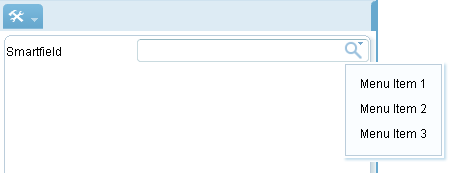
\includegraphics[width=0.8\textwidth]{smartfieldmenu.png}
\caption{Menus attached to a smart field.}
\label{fig:smartfield_menu}
\end{figure}

By default, the menus will only be shown if a value of the smart field has been selected. To show the menus even if the smart field is empty, one has to override the menu's \lstinline$getConfiguredEmptySpaceAction$ method:

\begin{lstlisting}[backgroundcolor=\color{white}]
@Override
protected boolean getConfiguredEmptySpaceAction() {
 return true;
}
\end{lstlisting}

% --------------------------------------------------------------------------- %
\section{List Box}
needs text

% --------------------------------------------------------------------------- %
\section{Tree Box}
needs text

% --------------------------------------------------------------------------- %
\section{Table Field}
needs text

\noindent Existing Documentation
\begin{itemize}
  \item wiki tutorial \url{http://wiki.eclipse.org/Scout/Tutorial/3.8/Minicrm/Table_Field}
  \item forum: \url{http://www.eclipse.org/forums/index.php/t/392053/}
  \item forum: load/save data \url{http://www.eclipse.org/forums/index.php/t/253311/}
\end{itemize}

% --------------------------------------------------------------------------- %
\section{Page Field}
needs text

\noindent Existing Documentation
\begin{itemize}
  \item forum: \url{http://www.eclipse.org/forums/index.php/t/395360/}
\end{itemize}

% --------------------------------------------------------------------------- %
\section{Image Field}
needs text

\noindent Existing Documentation
\begin{itemize}
  \item forum: scrollbars \url{http://www.eclipse.org/forums/index.php/t/291205/}
\end{itemize}

% --------------------------------------------------------------------------- %
\section{HTML Field}
needs text

% --------------------------------------------------------------------------- %
\section{Image Field}
needs text

% --------------------------------------------------------------------------- %
\section{SVG Field}
needs text

\noindent Existing Documentation
\begin{itemize}
  \item wiki tutorial \url{http://wiki.eclipse.org/Scout/Tutorial/3.8/SVG_Field}
\end{itemize}

% --------------------------------------------------------------------------- %
\section{Browser Field}
needs text

\noindent Existing Documentation
\begin{itemize}
  \item forum: \url{http://www.eclipse.org/forums/index.php/t/414483/}, 
  \item forum: \url{http://www.eclipse.org/forums/index.php/t/369963/}, 
  \item forum: mozilla as default: \url{http://www.eclipse.org/forums/index.php/t/342433/}
\end{itemize}

% --------------------------------------------------------------------------- %
\section{Calendar Field}
needs text

\noindent Existing Documentation
\begin{itemize}
  \item forum: calendar field \url{http://www.eclipse.org/forums/index.php/t/370052/}
  \item forum: execloaditems \url{http://www.eclipse.org/forums/index.php/t/277447/}
  \item forum: filtering items \url{http://www.eclipse.org/forums/index.php/t/285644/}
  \item forum: usage example \url{http://www.eclipse.org/forums/index.php/t/265028/}
\end{itemize}

% --------------------------------------------------------------------------- %
\section{File Chooser Field}
needs text

\noindent Existing Documentation
\begin{itemize}
  \item forum: file chooser field \url{http://www.eclipse.org/forums/index.php/t/377581/}
  \item forum: open with default file name: \url{http://www.eclipse.org/forums/index.php/t/351352/}
  \item how-to wiki: rap file chooser \url {http://wiki.eclipse.org/Scout/HowTo/3.8/Add_FileChooser_support_for_RAP_UI}
\end{itemize}

% --------------------------------------------------------------------------- %
\section{Master Slave Fields}
needs text

\noindent Existing Documentation
\begin{itemize}
  \item forum: \url{http://www.eclipse.org/forums/index.php/t/366931/}
\end{itemize}

% =========================================================================== %
\chapter{Custom Fields}
\chalabel{custom_fields}

needs text

\noindent Existing Documentation
\begin{itemize}
  \item how-to wiki: \url{http://wiki.eclipse.org/Scout/HowTo/3.8/Add_a_custom_GUI_component}
  \item forum: wrap existing javaview.de swing component \url{http://www.eclipse.org/forums/index.php/t/262755/}
\end{itemize}

  * concept
  * showcase: drawing application

% =========================================================================== %
\chapter{Template Fields}
needs text

\noindent Existing Documentation
\begin{itemize}
  \item concept wiki: \url{http://wiki.eclipse.org/Scout/Concepts/Template}
  \item forum: form data for template fields \url{http://www.eclipse.org/forums/index.php/t/261235/}
  \item forum: form ''modularisation'' \url{http://www.eclipse.org/forums/index.php/t/245857/}
\end{itemize}

% =========================================================================== %
\chapter{Bookmarks}
needs text

% =========================================================================== %
\chapter{Client Notification}
needs text

\noindent Existing Documentation
\begin{itemize}
  \item presentation: \url{http://wiki.eclipse.org/images/e/ea/20121022_BahBah_Slides.pdf}
  \item concept wiki: \url{http://wiki.eclipse.org/Scout/Concepts/Client_Notification}
  \item forum: \url{http://www.eclipse.org/forums/index.php/t/241053/}
\end{itemize}
      
% =========================================================================== %
\chapter{File Upload and Download}
needs text

\noindent Existing Documentation
\begin{itemize}
  \item how-to wiki: \url{http://wiki.eclipse.org/Scout/HowTo/3.8/Transfer_a_file_from_the_client_to_the_server}
  \item how-to wiki: \url{http://wiki.eclipse.org/Scout/HowTo/3.8/Use_RemoteFileService}
  \item forum with error message box exampl \url{http://www.eclipse.org/forums/index.php/t/441101/}
  \item forum: \url{http://www.eclipse.org/forums/index.php/t/368166/}
  \item forum: \url{http://www.eclipse.org/forums/index.php/t/366585/}
  \item forum: remotefileservice \url{http://www.eclipse.org/forums/index.php/t/266862/}
  \item forum: file download \url{http://www.eclipse.org/forums/index.php/t/263896/}
  \item forum: load \& display file \url{http://www.eclipse.org/forums/index.php/t/440934/}
\end{itemize}

% =========================================================================== %
\chapter{Application Branding}
needs text

\noindent Existing Documentation
\begin{itemize}
  \item forum: \url{http://www.eclipse.org/forums/index.php/t/373921/}
  \item forum: Splash \url{http://www.eclipse.org/forums/index.php/t/263003/}, 
  \item forum: Splash \url{http://www.eclipse.org/forums/index.php/t/164495/}
  \item forum: Login Box \url{http://www.eclipse.org/forums/index.php/t/417248/}
  \item forum: App Icon \url{http://www.eclipse.org/forums/index.php/t/263221/}
  \item forum: App Name \url{http://www.eclipse.org/forums/index.php/t/262121/}
  \item forum: Desktop \url{http://www.eclipse.org/forums/index.php/t/373921/}
  \item forum: Scout info form \url{http://www.eclipse.org/forums/index.php/t/236630/}
\end{itemize}

* Icons
* Fonts / Colors
* Look and Feel (Swing)

% --------------------------------------------------------------------------- %
\section{Rayo Look and Feel}
needs text

\noindent Existing Documentation
\begin{itemize}
  \item forum \url{http://www.eclipse.org/forums/index.php/t/369809/}
  \item wiki tutorial \url{http://wiki.eclipse.org/Scout/Tutorial/3.8/Rayo_Look_and_Feel}
\end{itemize}

% --------------------------------------------------------------------------- %
\section{Branding the Swing Client}
needs text

\noindent Existing Documentation
\begin{itemize}
  \item how-to wiki: for logo \url{http://wiki.eclipse.org/Scout/HowTo/3.8/Branding_the_Swing_Client}
  \item how-to wiki: app logo \url{http://wiki.eclipse.org/Scout/HowTo/3.8/Exchange_Default_Images}
\end{itemize}

% --------------------------------------------------------------------------- %
\section{Branding the SWT Client}
needs text

\noindent Existing Documentation
\begin{itemize}
  \item how-to wiki: for logo \url{http://wiki.eclipse.org/Scout/HowTo/3.8/Branding_the_Swing_Client}
  \item how-to wiki: app logo \url{http://wiki.eclipse.org/Scout/HowTo/3.8/Exchange_Default_Images}
\end{itemize}

% --------------------------------------------------------------------------- %
\section{Branding the Webclient}
needs text

\noindent Existing Documentation
\begin{itemize}
  \item forum \url{http://www.eclipse.org/forums/index.php/t/367983/}
\end{itemize}

% =========================================================================== %
\chapter{Advanced Topics}
needs text  

% --------------------------------------------------------------------------- %
\section{Modifying the UI at Runtime}
needs text

\noindent Existing Documentation
\begin{itemize}
  \item forum: inject fields in form \url{http://www.eclipse.org/forums/index.php/t/367124/}
\end{itemize}

% --------------------------------------------------------------------------- %
\section{Focus Handling}
needs text

\noindent Existing Documentation
\begin{itemize}
  \item forum: \url{http://www.eclipse.org/forums/index.php/t/369585/}
\end{itemize}

% --------------------------------------------------------------------------- %
\section{Keyboard Control}
needs text

\noindent Existing Documentation
\begin{itemize}
  \item forum: \url{http://www.eclipse.org/forums/index.php/t/351417/}
\end{itemize}

% --------------------------------------------------------------------------- %
\section{Master Detail Pages}
needs text

\noindent Existing Documentation
\begin{itemize}
  \item \url{http://www.eclipse.org/forums/index.php/t/405999/}
\end{itemize}

% --------------------------------------------------------------------------- %
\section{Client Only Applications}
needs text

\noindent Existing Documentation
\begin{itemize}
  \item how-to wiki: \url{http://wiki.eclipse.org/Scout/HowTo/3.8/Create_a_Standalone_Client_with_DB_Access}
  \item forum: client only \url{http://www.eclipse.org/forums/index.php/t/210183/}
  \item forum: offline capable client \url{http://www.eclipse.org/forums/index.php/t/210183/}
\end{itemize}


% --------------------------------------------------------------------------- %
\section{Headless Client}
needs text

\noindent Existing Documentation
\begin{itemize}
  \item headless client forum \url{http://www.eclipse.org/forums/index.php/t/262563/}
\end{itemize}

% --------------------------------------------------------------------------- %
\section{Client Startup}
needs text

\noindent Existing Documentation
\begin{itemize}
  \item reading command line parameters forum \url{http://www.eclipse.org/forums/index.php/t/281816/}
  \item do something right after login forum \url{http://www.eclipse.org/forums/index.php/t/261999/}
\end{itemize}

\subsection{Config.ini File}
needs text

\noindent Existing Documentation
\begin{itemize}
  \item config ini file forum \url{http://www.eclipse.org/forums/index.php/t/365140/}
  \item os independent *product/confg.ini forum \url{http://www.eclipse.org/forums/index.php/t/261674/}
\end{itemize}

% --------------------------------------------------------------------------- %
\section{Client Shutdown}
needs text

% --------------------------------------------------------------------------- %
\section{Threading and Jobs}
needs text

\noindent Existing Documentation
\begin{itemize}
  \item threading and jobs concept wiki \url{http://wiki.eclipse.org/Scout/Concepts/Client_Plug-In#Threading_and_Jobs}
\end{itemize}


% --------------------------------------------------------------------------- %
\section{Caching}
needs text

% --------------------------------------------------------------------------- %

\ifx\wholebook\relax\else
   \begin{thebibliography}{99}
  \addcontentsline{toc}{chapter}{Bibliography}
  
  % add/insert books in alphabetical order of 1st author
  
  \bibitem{batessierra05}
    \textit{Bert Bates, Kathy Sierra},
	\textbf{Head First Java} 2nd edition, 
	O'Reilly Media, 2005.

  \bibitem{bloch08} 
    \textit{Joshua Bloch},
    \textbf{Effective Java} 2nd edition, 
	Addison-Wesley, 2008.
	
  \bibitem{eckel06}
    \textit{Bruce Eckel},
	\textbf{Thinking in Java} 4th edition, 
	Prentice Hall International, 2006.

\end{thebibliography}

   \end{document}
\fi

% =========================================================================== %
